% File: tex/cygnus.tex
% Author: Timo L. R. Halbesma <timo.halbesma@student.uva.nl>
% Version: 0.01 (Initial)
% Date created: Thu Sep 01, 2016 01:56 AM
% Last modified: Mon Sep 05, 2016 01:59 AM
%
% Description: Masterthesis, Observational Overview of extended Cygnus emission


\documentclass[MScProj_TLRH_ClusterEnergy.tex]{subfiles}

\begin{document}
\chapter{Observational Overview of the Cygnus Cluster}
\label{sec:cygnus}

The Cygnus constellation, denoted by the symbol `Cyg'
\citep{1922PA.....30..469R}, is found on the Northern hemisphere right in the
plane of the Milky Way, just below the well-studied Kepler Field. More
quantitatively, it is located at a declination of roughly $+27^\circ < \delta <
+54^\circ$ and a right ascension $19^{\rm h}17^{\rm m} < \alpha < 21^{\rm
h}45^{\rm m}$. The constellation was named `The Swan' by ancient Greek
astronomers and is featured as early as Ptolemy's list of constellations. The
constellation has stars well visible to the naked eye, such as its brightest
star at the tail of the Swan, Deneb ($\alpha$ Cyg, also part of the asterism
Summer Triangle together with Vega and Altair), and at the head the
optical double Albireo ($\beta$ Cyg and $\beta_2$ Cyg). The
constellation hosts interesting deep-sky objects like the Veil nebula, a large
bright feature in the X-ray sky caused by a supernova explosion. Other
well-known, well-studied X-ray objects found in Cygnus are the (galactic) X-ray
binary Cyg~X-1, widely accepted as the first (indirect) proof of the existence of black
holes, and the microquasar Cyg~X-3 where a Wolf-Rayet is found in a binary with a 
compact object. Figure~\ref{fig:CygAMilkyway} shows this part of the sky.

\begin{figure}
\centering
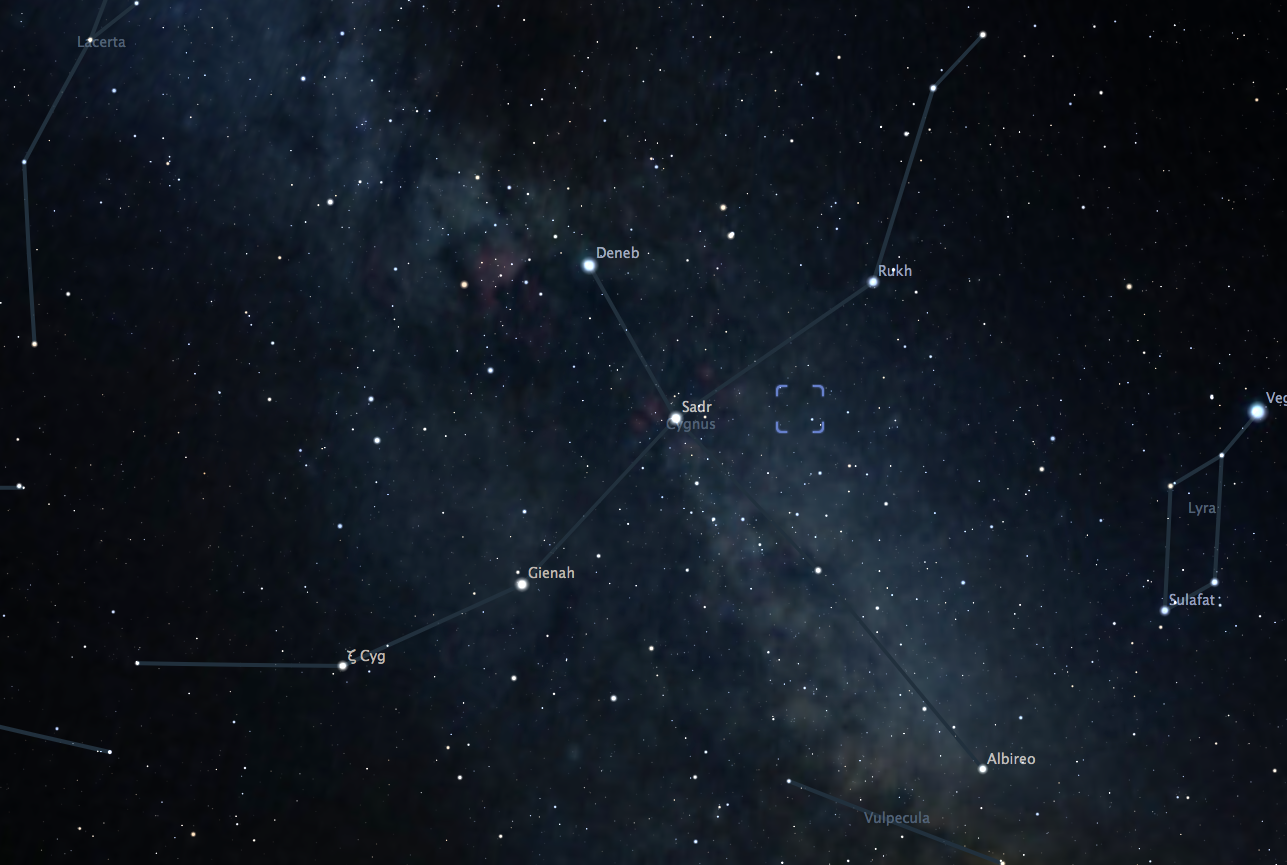
\includegraphics[width=0.78\textwidth]{introduction/CygA.png}
\caption{Cygnus, the Swan constellation, is found in the plane of the Milky Way
         on the Northern hemisphere. The square indicates the location of Cygnus~A.
         TODO: use clearer image, e.g. amateur astronomer photo?}
\label{fig:CygAMilkyway}
\end{figure}
%   \begin{figure}
%   \centering
%   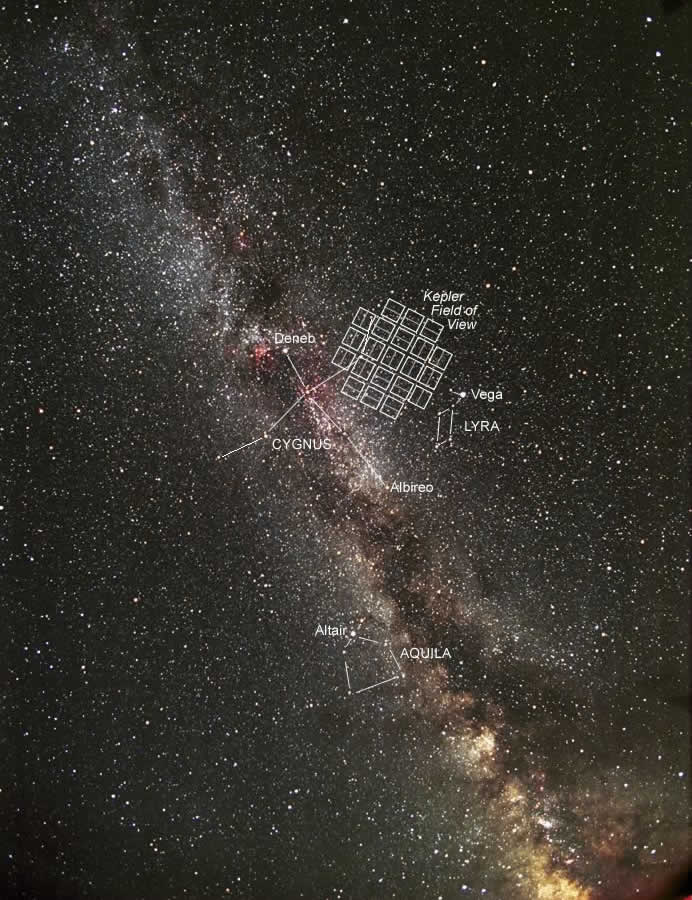
\includegraphics[width=0.78\textwidth]{/introduction/KeplerFOV_JustAboveCygnusConstellation.jpg}
%   \caption{TODO: Do I even want to show this?}
%   \label{fig:MilkyWay_Kepler}
%   \end{figure}%   

Trough out this thesis we use the name Cygnus~A for the radio source as well as 
for its optically visible host galaxy. In addition, the cluster of galaxies is 
also named Cygnus~A. This indicates that one cannot think of the object Cygnus~A 
as just one source. To avoid confusion we will indicate which source of emission
is meant such that the radio source means the AGN, the cD galaxy means the optical
galaxy, and the cluster or X-ray source means the emission from the intra cluster 
medium. The literature overview in this section does not include the literature 
on the majority of the radio emission, neither on most of the optical emission, 
nor the majority of X-ray studies that focus on the emission in the core, unless 
relevant to our merger study. Seminal publications in the field of radio astronomy
are bundled in \citet{1982cra..book.....S} and contain very interesting early 
literature on the strong radio source Cygnus~A. In addition, proceedings of a 
four day workshop on Cygnus~A by \citet{1996cyga.book.....C}, and the 
comprehensive review by \citet{1996A&ARv...7....1C} provide a great source of 
information on prior observations of Cygnus~A as these publications and 
references therein provide an overview of the study of Cygnus~A up to mid 1995 
in all frequency domains of the electromagnetic spectrum. Our overview does 
include X-ray observations of the extended source published to date spanning from
early \satellite{Uhuru} up to curent-day \satellite{Chandra} observations 
including the ongoing multi-wavelength campaign of Wise and collaborators. 

However, we cannot discuss Cygnus~A without at least showing the well-known 
radio observation. Perhaps most astronomers know Cygnus~A as one of the most 
powerful radio sources in the sky, the brightest extragalactic source, the 
classical radio double, the archetype of the FR-II class \citep{1974MNRAS.167P..31F}
of radio galaxies (Figure~\ref{fig:CygA_Radio}). The extreme brightness of the 
radio source can clearly be seen in Figure~\ref{fig:CygA_Radio_bright}. Although 
found at a redshift $z=0.562$ \citep{1997ApJ...488L..15O},
Cygnus~A is as bright as a $z=1$ source, and a thousand times brighter than any
other source at the same distance \citep{1996cyga.book....1S, 1996A&ARv...7....1C}.
It is of no surprise that the radio emission is detected as early as the first radio
observations were carried out by radio astronomy pioneer Grote Reber
\citet{1944ApJ...100..279R, reber1948cosmic}. On a side note, radio astronomers 
that do not study Cygnus~A might rather dislike the radio source as it so bright
it usually ends up in the sidelobes of modern radio telescopes and explicitly has
to be filtered out of the correlated data \citep[e.g.][]{2012MNRAS.422..563O}. A
few years later \citet{1954ApJ...119..206B} report that photographic plates of the
same part of sky reveal a few galaxies clustered together at a position corresponding
with the location of the radio source. We now move away from the radio source
and consider the large, diffuse X-ray emission featured in the first catalog 
of X-ray sources seen by the \satellite{Uhuru} satellite \citep{1972ApJ...178..281G}. 

\begin{figure}
\centering
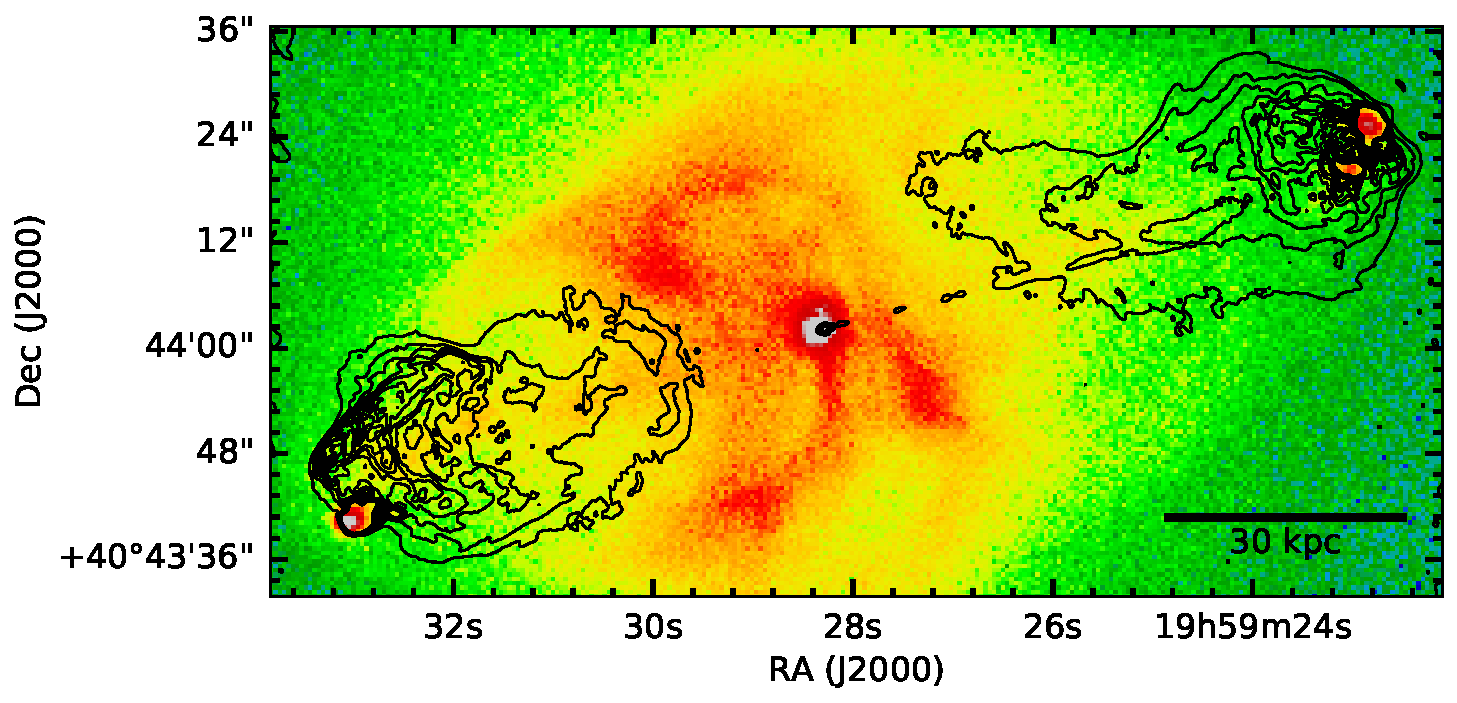
\includegraphics[width=\textwidth]{introduction/radio/CygA_Radio_5GHz.pdf}
\caption{JVLA observation at 5~GHz, 0.5'' resolution of Cygnus~A.
         The collimated outflow from a central source is visible. The jet injects 
         relativistic electrons, and deposits energy in the medium surrounding the 
         brightest cluster galaxy. The giant radio lobes are clearly visible, and hot
         spots can be seen slightly albeit misaligned with the direction of the jet.
         Figure reproduced from \citet{1996A&ARv...7....1C}.}
\label{fig:CygA_Radio}
\end{figure}

\begin{figure}
\centering
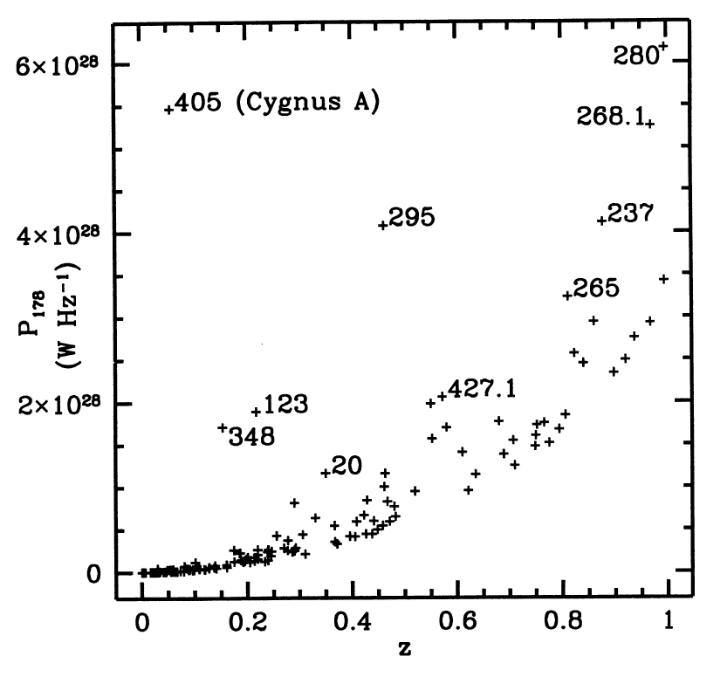
\includegraphics[width=0.78\textwidth]{introduction/radio/RadioPowerRedshift3C405IsOutlier.png}
\caption{Radio sources at 178 MHz (apart from quasars) in the revised third
         Cambridge catalog (3CR) with a redshift below $z=1$. Note that the
         radio power of 3C~405 (Cygnus~A) is significantly higher than galaxies
         at similar (low) redshift. Figure adopted from \citet{1996cyga.book....1S}.}
\label{fig:CygA_Radio_bright}
\end{figure}

After each discovery an initial debate sprouted within the community regarding 
(i) the origin, (ii) emission mechanism, and (iii) the possible, exciting
connections between two or three of the sources of unexplained emission.
The debate has now mostly settled and consensus has been reached that Cygnus~A
is indeed the BCG hosting an AGN within a cluster of galaxies. The details,
however, are still subject to several major studies. Cygnus~A is an excellent
target to study AGN~feedback, a merging cluster of galaxies, the interplay between
both, and the contribution both physical processes have on heating the hot intra
cluster medium, as outlined in section~\ref{sec:outline}. The brightness and proximity
allow for unprecedented spatial and spectral resolution to reveal insight into
the detailed workings of AGN~Feedback. An even more intriguing feature, however, 
is not the highly fascinating active galactic nucleus. Rather, we take a specific 
interest in the cluster of galaxies Cygnus~A is part of as it is currently 
undergoing a major, disruptive merger with a subcluster. This is not a well-known
observation because the majority of studies focusses on the central region where
the AGN~feedback can be studied. Furthermore, in order to see the diffuse
emission to the North West of Cygnus~A, the infalling sub-cluster, one has to 
smoothen the emission significantly (Figure~\ref{fig:CygA_Xray_extended}).

A summary of previous X-ray observations presented in Table~\ref{tab:xray_extended}, 
and an overview of optical studies given in Table~\ref{tab:relevant_optical}. 
Certain references are of particular interest or contain figures that we explicitly
adopt in the paragraphs following the tables.

\newpage
\begin{landscape}
\pagestyle{plain}
\captionsetup{font=normalsize}

\setlength\LTleft{-25pt}
\setlength\LTright{0pt}
\begin{longtable}{@{\extracolsep{\fill}}lp{\textwidth}p{0.36\textwidth}@{}}
\caption{Overview of the literature on the extended emission in the Cygnus~A cluster
         \label{tab:xray_extended}} \\
\hline
Observatory & Conclusions & Reference  \\
\hline \endfirsthead
\caption{Overview of the literature on the extended emission in the Cygnus~A cluster (continued from previous page)} \\
\hline
Observatory & Conclusions & Reference  \\
\hline \endhead

\hline \multicolumn{3}{c}{{Table continues on next page}} \\ \hline
\endfoot

\hline \hline
\endlastfoot
     
\satellite{Uhuru} & 
Detection of extended source with $0.270$ square degrees area. Suggested counterpart CygA. 
& \citet{1972ApJ...178..281G} \\

\satellite{Copernicus}  & 
Confirmation X-ray source has powerful radio galaxy CygA as counterpart. 
Thermal bremsstrahlung emission mechanisms suggested, although still uncertain. 
&  \citet{1974MNRAS.168..479L}  \\

\satellite{ANS}  & 
Misalignment peak of X-ray emission and radio galaxy by $6$' if assumed a point source.
On the other hand, consistent with $>12$' extended emission as expected from hot cluster gas.
& \citet{1977ApJ...214...35B} \\

\satellite{HEAO-1} & 
Extended \mytilde $2$' source with a complex geometry. Fit of isotermal sphere model yields
a core radius of $0.19$ Mpc and central density of $0.014$ cm\Sup{-3}. 
A total mass for the galaxy Cygnus~A is estimated to be $10^{14}$ M\Sun.
& \citet{1979ApJ...230L..67F} \\

\satellite{Einstein} & 
The X-ray emission is extended, spherically symmetric and centered on the cD galaxy. 
& \citet{1980HiA.....5..695F} \\

\satellite{Ariel-V} &
Catalog entry: consistend with prior literature, and detection of iron K$\alpha$ line.
& \citet{1984AandAS...56..415B} \\

\satellite{Einstein} (2) & 
Cooling flow of $90$ M\Sun yr\Sup{-1}. Mass-estimate of $10^{14}$ M\Sun (King
approximation) adopting the \satellite{HEAO-1} value
for the core radius $r_c = 0.2$ Mpc) within a source that extends North West from
the central radio source by over $1$~Mpc ($H_0 = 50$ km/s/Mpc).
& \citet{1984MNRAS.211..981A} \\

\satellite{Exosat} & 
Iron K$\alpha$ detection. Highly absorbed power-law component associated with nucleus of the radio source. 
The source extends significantly to the North West, and the central density is $0.02$ cm\Sup{-3}.
& \citet{1987MNRAS.227..241A} \\

\satellite{Ginga} & 
The X-ray spectrum shows a thermal component with K-shell transition lines and a highly absorbed power-law. 
The former is consistent with hot intra cluster gas, and the latter suggests Cygnus~A hosts an obscured quasar.
& \citet{1994ApJ...431L...1U}  \\

\satellite{ROSAT} HRI & 
The X-ray structure is dominated by the cluster emission centered on the galaxy Cygnus~A.
A modified King (beta-model, equation~\eqref{eq:betamodel})model yields a core radius of 
$35 \pm 5$ arcsec, central density of $0.07\pm 0.02$ and King-model index of 
$\beta=0.75 \pm 0.25$. Note that only the inner $100$ kpc is observed.
& \citet{1994MNRAS.270..173C} \\

\satellite{ROSAT} PSPC &
The X-ray emission is dominated by the thermal emission from the hot ICM, agrees reasonably well
with spherically symmetric emission within the inner 5 arcsec, and is strongly peaked on the central galaxy.
A lower temperature towards the center of the gravitational potential is observed from which 
a cooling flow of $250$ M\Sun \, yr\Sup{-1} is induced with a cooling radius of $180$ kpc. 
A plume extending a bit over $15$ arcmim to the North West is reported, and the possibility of a past or
ongoing cluster-cluster merger is suggested. Central density is $0.03$ cm\Sup{-3}.
& \citet{1996MNRAS.278..479R} \\

\satellite{ASCA} & 
The merger geometry appears very straightforward. A temperature jump is observed in the
region between Cygnus~A and the subcluster to the North West. The temperatures measured
are $T_0 \approx 4 \pm 1$ K, and postshock $T_1 \approx 8_{-1}^{+2}$ K,
and the estimated merger velocity is $2000$ km/s. NB, the authors assume $H_0 = 50$ km/s/Mpc.
& \citet{1999ApJ...521..526M}  \\

%\satellite{XTE} & & \\
%\satellite{AXAF} & & \\

\satellite{Chandra} &
Part one and two of a series of publications on Cygnus~A, the scope of these publications 
is the emission from the hotspots, respectively, the nucleus. Included for completeness,
but outside the scope of our overview.
& \begin{tabular}[t]{@{}c@{}} \citet{2000ApJ...544L..27W} \\ \citet{2002ApJ...564..176Y} \end{tabular}  \\

\satellite{Chandra} (2) &
First mention of emission to the North West likely due to another cluster.
The mass derived from hydrostatic equilbrium (equation~\eqref{eq:hydrostaticmass}) 
within $500$ kpc (assuming $H_0 = 50$ km/s/Mpc) is $2 \times 10^{14}$ M\Sun \,
respectively $2.8 \times 10^{14}$ M\Sun \, for constant and centrally decreasing
temperature profiles, and the total mass from the X-ray emitting gas
is $1.1 \times 10^{13}$ M\Sun. An isothermal beta model is fitted and yields 
$r_c \approx 18$ arcsec and $\beta \approx 0.51$. & \citet{2002ApJ...565..195S} \\

%\satellite{Astro-E} & & \\

\satellite{Suzaku} &
A temperature jump is observed between Cygnus~A and the subcluster to the North West.
Combined with redshift measures of the iron K line the system appears to have 
a simple geometry. Both clusters merge at a velocity of $2400-3000$ km/s, and
the projection angle is estimated as 54$^\circ$.
& \citet{2013AN....334..346S}  \\

\satellite{Chandra} (3) & Nicely summarises \satellite{Chandra} observations of the
central region prior to the \citet{2014cxo..prop.4448W} observations. Outside 
the scope of this overview as it focusses mainly on the central region.
& \citet{2015IAUS..313..236N} \\

\satellite{Chandra} (4) &
X-ray observations as part of an ongoing multi-wavelength observational campaign
that provides the dataset used to constrain the initial conditions for the 
numerical simulations in this thesis.
& \citet[in prep]{2016MNRAS.123..456W} \\
\end{longtable}
\newpage
\begin{longtable}{@{\extracolsep{\fill}}lp{\textwidth}p{0.36\textwidth}@{}}
\caption{Overview of cluster or merger relevant optical studies of Cygnus~A cluster
         members \label{tab:relevant_optical}} \\
\hline
Observatory & Conclusions & Reference  \\
\hline \endfirsthead
\caption{Overview of cluster or merger relevant optical studies of Cygnus~A cluster
         members (continued from previous page)} \\
\hline
Observatory & Conclusions & Reference  \\
\hline \endhead

\hline \multicolumn{3}{c}{{Table continues on next page}}  \\ \hline
\endfoot

\hline \hline
\endlastfoot
     
Palomar & The 200 inch Palomar telescope shows the brightest member of a cluster of galaxies
coincides with the location on the sky of the powerful radio galaxy Cygnus~A.
& \citet{1954ApJ...119..206B} \\

Kitt Peak: Lick & 
Cygnus~A lies in the plane of the Milky Way (Figure~\ref{fig:CygAMilkyway}), thus 
the Galaxy conceals the majority of the galaxies in the cluster. The authors
conclude that the cluster Cygnus is Abell-poor based on the observation of a mere
five galaxies. The BCG Cygnus~A can be classified as a cD galaxy, and the measured
velocity dispersion is $2000 \pm 500$ km/s.
& \citet{1982MNRAS.200..153S} \\

Kitt Peak: Steward & 
Velocities of 41 galaxies associated with the cluster are observed. The authors conclude
the Abell richness of the cluster is 1 up to 4. A relatively high velocity dispersion of
$1581^{+286}_{-197}$ is reported, and the dynamical center of the spatial distribution of 
galaxies appears shifted to the North West, thus CygA is not located at the center of a 
rich cluster of galaxies. Although statistical evidence supporting two 
distinct clusters is rather weak, such high velocity dispersions are typically found in 
clusters with two or more subclusters.
&  \citet{1997ApJ...488L..15O} \\

Kitt Peak: WIYN &
Detection of 77 additional galaxies associated with the cluster, combined with temperature
structure inferred from X-rays, allows for dynamical modelling. This shows the optical
distribution of galaxies and the temperature structure is consistent with a cluster-cluster
merger 0.2-0.6 Gyr prior to core passage projected at an angle of $30^{\circ}-45^{\circ}$.
& \citet{2005AJ....130...47L} \\
\end{longtable}

\end{landscape}
\newpage

An overview of X-ray observations with different instruments in the first couple
of years is shown in Figure~\ref{fig:uhuru_copernicus_ans_heao}, where the location
of the radio source (3C~405) is marked with a cross. This is compelling evidence 
suggesting an apparent connection between the radio source and the X-ray emission.

\begin{figure}
\centering
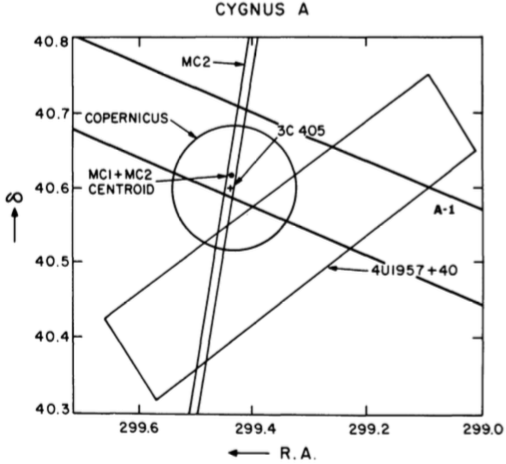
\includegraphics[width=0.78\textwidth]{introduction/xray/Uhuru_Copernicus_HEAO.png}
\caption{Observed Cygnus~A cluster region with \satellite{Uhuru} (squared box), 
         \satellite{Copernicus} (sphere), \satellite{ANS} and \satellite{HEAO}
         (MC1, MC2). The radio galaxy is indicated with a cross (3C~405). Figure
         adopted from \citet{1979ApJ...230L..67F}}
\label{fig:uhuru_copernicus_ans_heao}
\end{figure}

A bit over a decade after the initial \satellite{Uhuru} discovery, consensus has
been reached regarding the emission mechanism of hot intra cluster gas 
\citep[e.g.][]{1977ARA&A..15..505B}. For Cygnus~A, \citet{1984MNRAS.211..981A}
are the first to write it is safe to assume thermal bremsstrahlung as main
emission mechanism, as first suggested by \citet{1974MNRAS.168..479L},
with additional iron K$\alpha$ line emission \citep{1984AandAS...56..415B,
1987MNRAS.227..241A}. In general, models of the emission originating from a spherically
symmetric distribution of gas in the gravitational potential of the cluster 
agree well with the observations \citep[e.g.][]{1978A&A....70..677C}.
\citet{1979ApJ...230L..67F} report similarities of Cygnus~A and its larger cluster
environment with M87 in the Virgo \citep{1978ApJ...219..413M} cluster, and with 
NGC~1275 in the Perseus cluster \citep{1978ApJ...224..718G}, and therefore 
fit the extended X-ray flux with an isothermal hydrostatic sphere model following 
\citet{1978ApJ...219..413M}. This yields first mass estimates of the cluster gas 
as well as values for the core radius and central density. For Cygnus~A this 
fit yields a total mass of
$10^{14}$ M\Sun, a temperature of $6.5$~keV, a central number density of
$0.014$ cm\Sup{-3} and luminosity of $4.7\cdot 10^{44}$ ergs s\Sup{-1} $(2-6
)$~keV. The model does require refueling as the cooling time is of order 3
billion years, which is smaller than the Hubble time. One of the major
problems in clusters of galaxies is the so-called cooling flow problem.

Although the emission mechanism has been found, the origin of the hot intra cluster
remains a mystery. Perhaps the gas simply fell into the cluster from a general inter
cluster medium \citep{1975PThPh..53..646T}, it might have been expelled by the galaxies
\citep{1973ApJ...185..787Y}. Another mystery remains heating and cooling of the gas.
The gas is thought to remain as hot as observed by means of shock heating, but at the same
time the central regions of clusters are observed to cool down.
Clusters of galaxies are assumed in hydrostatic equilibrium, thus virial theorem
requires an increase in central density as radiative losses actively cool the
cores of clusters of galaxies. Alternatively, one can think of this increase in
central density as mass flowing from the cluster outskirts to the bottom of the
potential well in its center \citep[e.g.][]{1977MNRAS.180..479F}. This cooling
flow problem is the main interest of \citet{1984MNRAS.211..981A}, specifically
to find observational evidence for these cooling flows. 

\begin{figure}
\centering
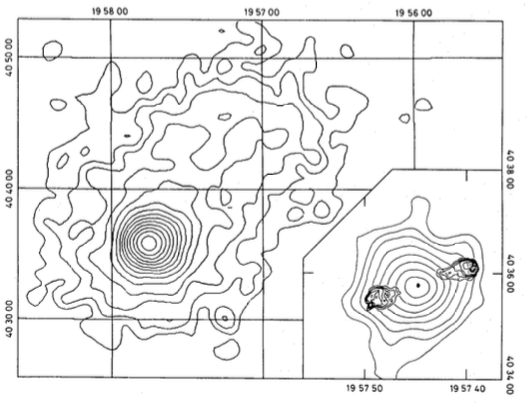
\includegraphics[width=0.78\textwidth]{introduction/xray/Einstein_CygA_Extended.png}
\caption{X-ray surface brightness observed with the \satellite{Einstein} satellite.
         The larger image shows the IPC observation smoothed with a 32" Gaussian, 
         and the inset shows 12" Gaussian smoothed HRI data with a 5 GHz radio 
         contour map of \citet{1984MNRAS.209..851A}. This observation clearly shows that 
         the classical radio double is found inside a cluster environment that extends
         significantly to the North West. Figure adopted from \citet{1984MNRAS.211..981A}.}
\label{fig:einstein_extended_radio_double}
\end{figure}

At this time the central galaxy is considered the archetype of a classical radio
double \citep[e.g.][]{1980MNRAS.192..931W}, and from photographic and spectroscopic
observations \citet{1982MNRAS.200..153S} find cD galaxy Cygnus~A to lie in a poor
cluster of galaxies. The authors also note a velocity dispersion of 2000 $\pm$ 500
km/s, although this study is based on a mere 5 galaxies. This makes Cygnus~A rather
exceptional as few other classical double radio galaxies are found within a cluster 
of galaxies. \citet{1984MNRAS.211..981A} are the first to show a clear image of the
large-scale emission smoothed with a 12'' Gaussian (Figure~\ref{fig:einstein_extended_radio_double}).
However, no significant peak to the North West has been observed yet, but these data
do show the emission extends significantly in this direction.
The large-scale emissions reaches over a mega parsec from the radio galaxy,
which is consistent with observations of other large clusters of galaxies.
Using the cooling flow model of \citet{1977MNRAS.180..479F}, it is found that the 
cooling rate is 90 M\Sun \, per year in the inner 125 kpc region. This shows that 
even poor clusters of galaxies can be powerful X-ray emitters and show clear signs
of cooling flows. Interestingly, Cygnus~A is the first classical double that not 
only lies in a cluster of galaxies but also shows clear signs of a cooling flow. \\

In the early nineties the improved spatial resolution of the High Resolution Imager
onboard \satellite{ROSAT} reveals a wealth of structure in the inner \mytilde $100$ arcsec
of Cygnus~A. On the larger scale, the \satellite{ROSAT} data does reveal a plume to the
North West. This feature shows the cluster medium is not relaxed and could be
interpreted as a sign either past or perhaps ongoing cluster-cluster merger activity.
\citet{1994MNRAS.270..173C} show that thermal emission associated with 
the cluster of galaxies peaks on the center of the Cygnus~A galaxy. The best-fit
modified King (beta-model, equation~\eqref{eq:betamodel}) model gives a central
density $n_0 = 0.07 \pm 0.02$ cm\Sup{-3}, with core radius $r_c = 35 \pm 5$ 
arcsec and King-model index $\beta = 0.75 \pm 0.25$.

We now briefly broaden our scope to highlight the basic structure seen in the direct
surroundings of the classical radio double CygA. The model for the extended emission 
is subtracted from the observed data and shows departures from spherical symmetry in
the central region as a result of interactions of the central radio source with the 
surrounding hot intra cluster gas in the form of excess X-ray
emission coinciding with radio hot spots, residual emission from the nucleus, a lower surface
brightness in regions associated with the inside of the radio lobes, and knots of excess
X-rays produced along some edges of the radio lobes. These features are clear signs of 
interactions of the radio jets with the intra cluster medium. In particular, the deficits 
within the radio lobes combined with excess at the edges is considered strong observational 
evidence in support of the basic jet model for powerful radio galaxies,
first suggested by \citet{1973MNRAS.164..243L, 1974MNRAS.166..305H}, worked out in detail by
\citet{1974MNRAS.169..395B, 1974MNRAS.166..513S} and reviewed by \citet{1984RvMP...56..255B}.
In this model an optically visible galaxy could have relativistic outflow from the center. 
These jets then cause cavities in the surrounding medium as relativistic material efficiently 
displaces the intra cluster medium, and jet termination by a strong shock causes heating visible 
as the hot spots. The radio lobes are advancing supersonically, thus, they must be preceded
by a strong shock in the ICM. As a result, the radio lobes are emptied of
thermal material \citep{1987ApJ...316..611D}. It seems that from this point in time 
onwards it is considered essential to observe clusters of galaxies both in radio and in
X-ray to study these processes in detail, and preceding observational campaigns usually
comprise of observations in both regimes. This leads to a model for the central
region shown in Figure~\ref{fig:JetModel} and Figure~\ref{fig:CygAJetsColour}. 

\begin{figure}
\centering
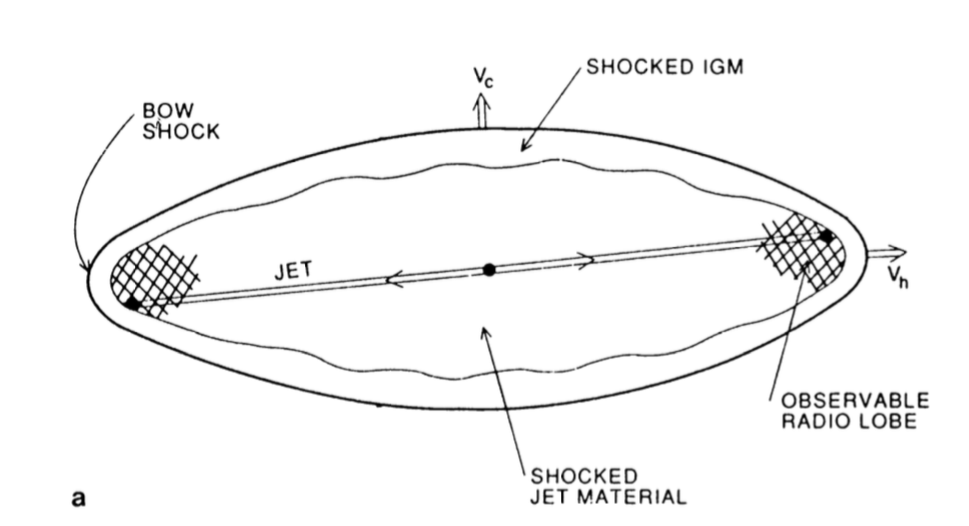
\includegraphics[width=0.87\textwidth]{introduction/xray/CocoonShock_Model.png}
\caption{This schematic representation shows features arising from interactions
         of jet outflow into ambient gas, as can be expected for the collimated 
         outflow of Cygnus~A into the intra cluster medium in the central region
         of the cluster it resides in. Figure adopted from \citet{1996A&ARv...7....1C},
         who reproduced it from \citet{1989ApJ...345L..21B}.}
\label{fig:JetModel}
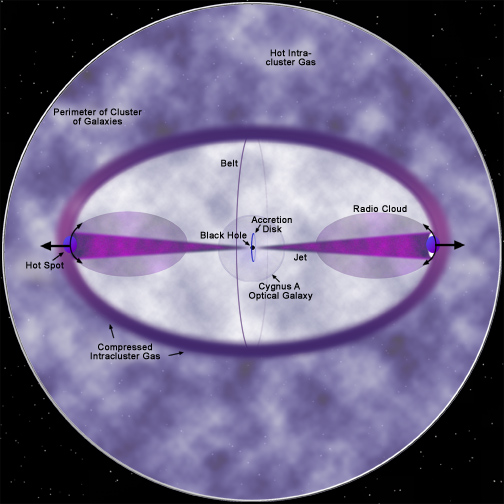
\includegraphics[width=0.87\textwidth]{introduction/cyg_illustration.jpg}
\caption{Schematic drawing of the central region of Cygnus~A. Here one can see
         the effect of jet outfow onto the intra cluster medium as can be seen
         in the innermost kpc surrounding the central galaxy of the cluster. 
         Image credit \citet{CygASchematic}.}
\label{fig:CygAJetsColour}
\end{figure}

Around the turn of the century optical imaging and spectroscopy shows that Cygnus~A 
lies in an extensive cluster of at least Abell richness 1, but possibly as high as 4
\citep{1997ApJ...488L..15O}. Improved optical observatories now make it possible to
detect significantly more galaxies associated with the cluster of galaxies Cygnus~A.
In previous observations the coincidence of the Cygnus cluster with the Milky Way 
obscured quite a lot of the rather faint galaxies. The authors report that
the velocity distribution appears bimodal (Figure~\ref{fig:velocityDispersion}) and note 
that the dynamical center of the spatial distribution appears somewhat to the northwest
(Figure~\ref{fig:velocityDistribution}).
The statistical evidence however, makes a rather weak case for the presence of two distinct
clusters. In totality, the system shows a high velocity dispersion of $1581^{+286}_{-197}$
km s\Sup{-1} which is typically so for clusters made up of two or more sub-clusters.

\begin{figure}
\centering
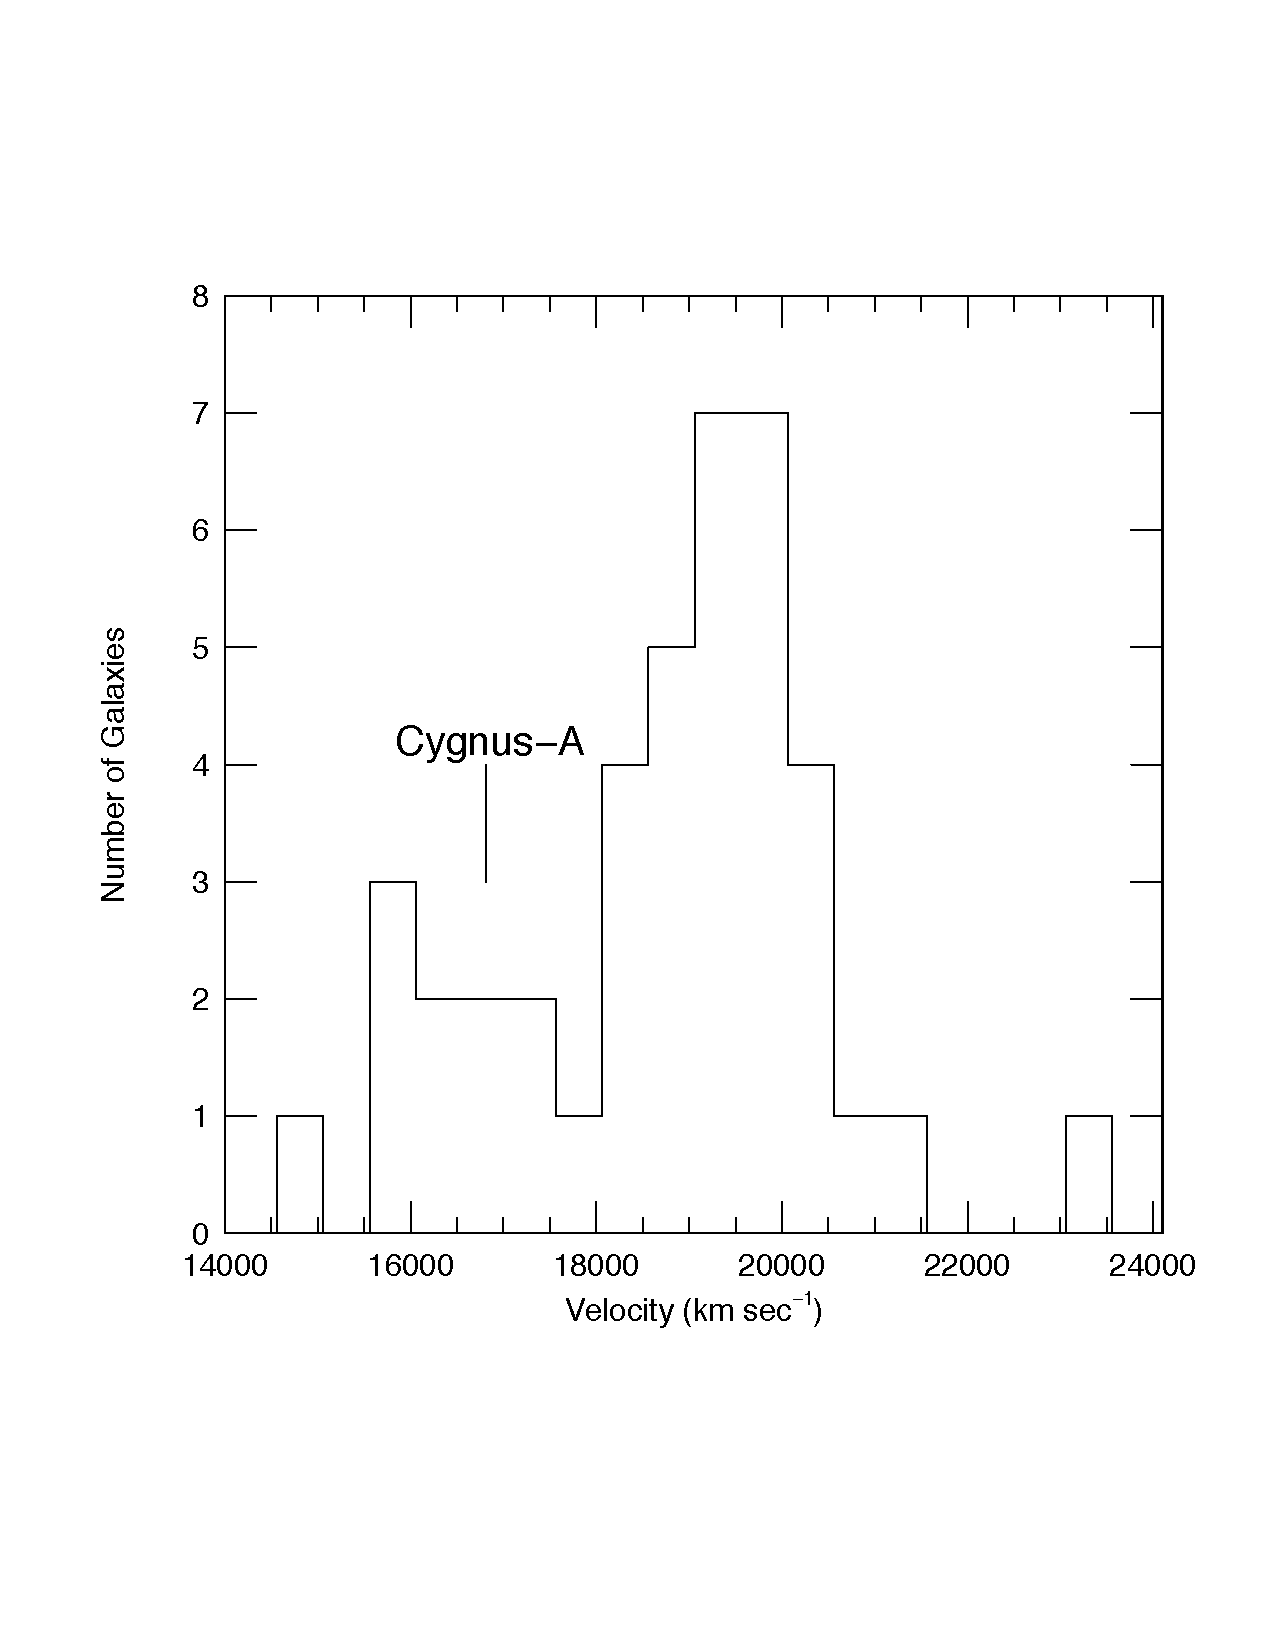
\includegraphics[width=0.74\textwidth]{introduction/optical/CygA_VelocityDispersion_1997.pdf}
\caption{Histogram showing the radial velocities obtained for 41 galaxies part of the 
         Cygnus~A cluster by \citet{1997ApJ...488L..15O}. Although a bimodal distribution
         is observed, the statistical evidence for two distinct clusters is weak. The
         high velocity dispersion, on the other hand, is typical for clusters consisting
         of two or more sub-clusters.}
\label{fig:velocityDispersion}
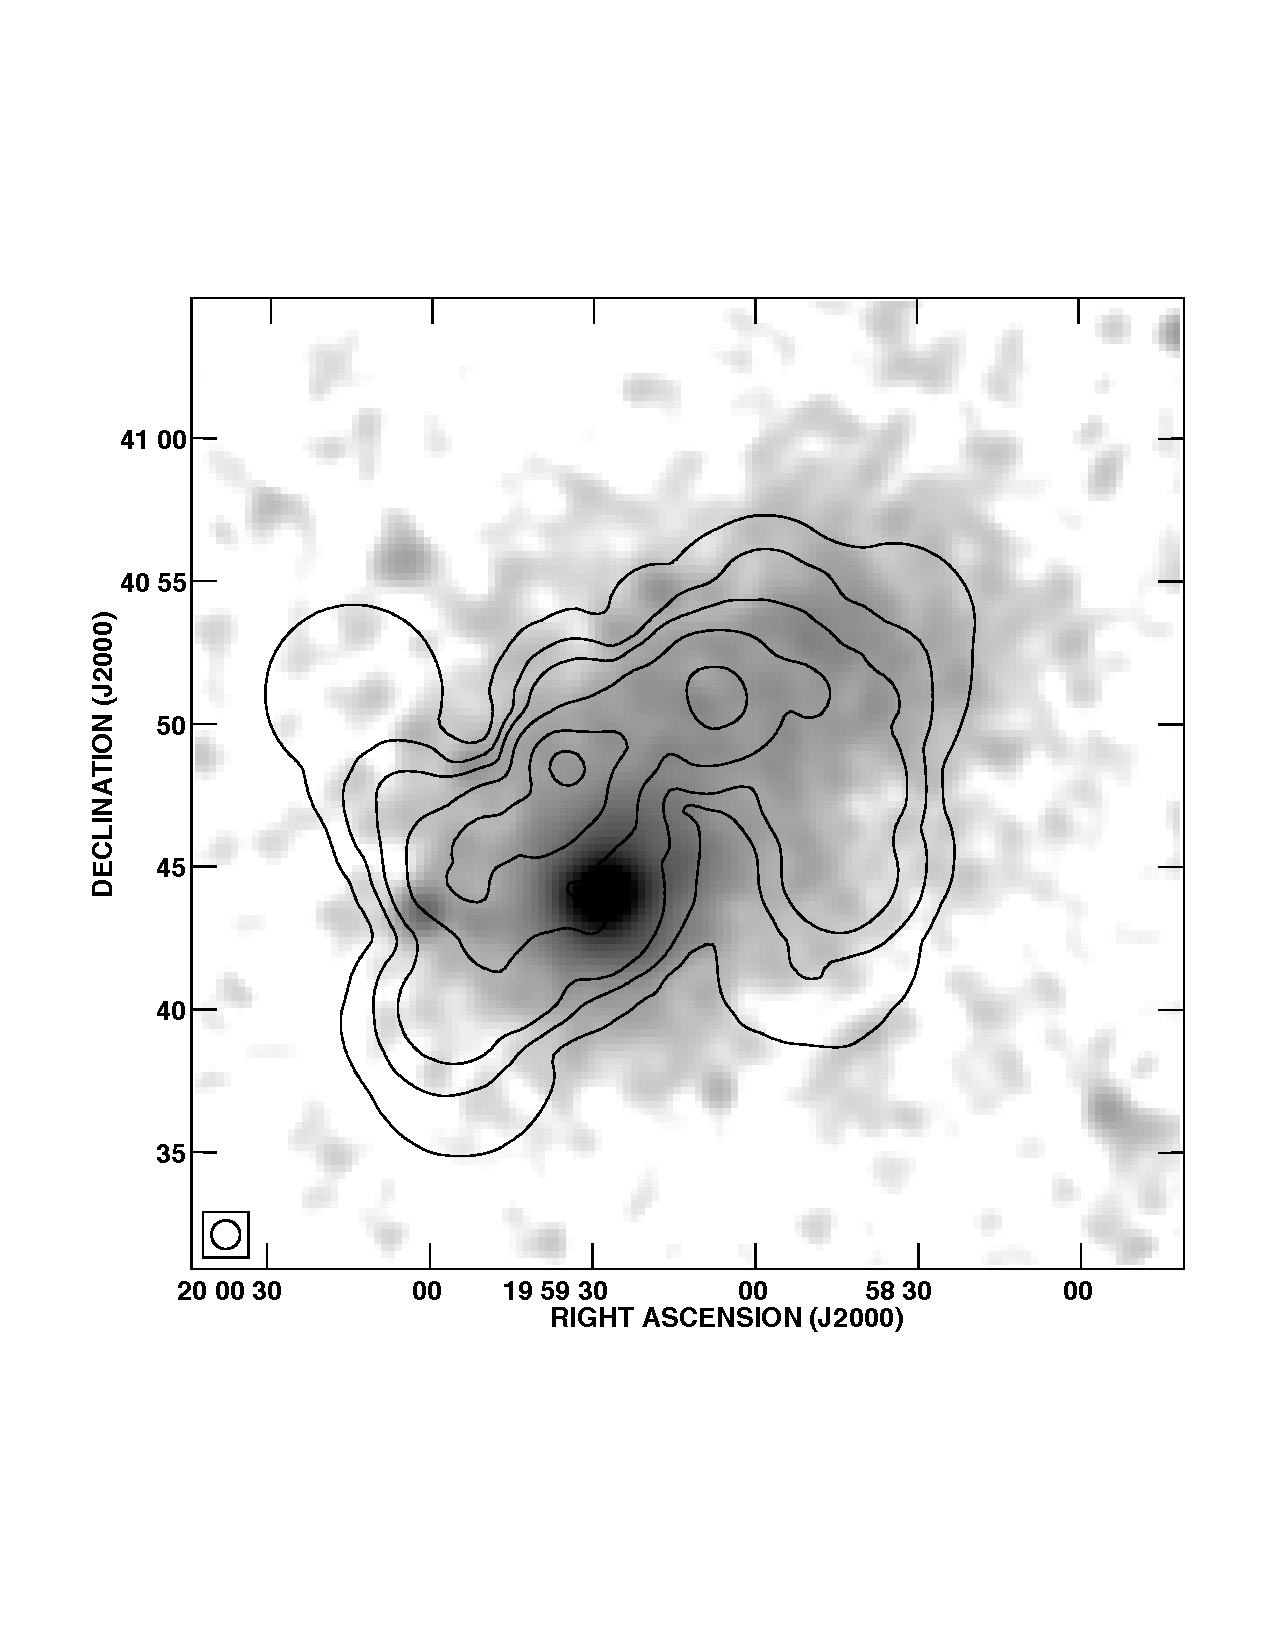
\includegraphics[width=0.7\textwidth]{introduction/optical/VelocityDistribution_1997.pdf}
\caption{The contour overlay shows the adaptively smoothed galaxy distribution
         centered on the dynamical center of mass overplotted on the \satellite{ROSAT}
         PSPC X-ray observation \citep{1996MNRAS.278..479R}. CygA is located at the
         brightest source of X-ray emission. Figure adopted from \citep{1997ApJ...488L..15O}. }
\label{fig:velocityDistribution}
\end{figure}

Back to the X-rays, \citet{1999ApJ...521..526M} interprete a temperature jump 
in the region between Cygnus~A and the North West plume seen in \satellite{ASCA} 
observations (Figure~\ref{fig:ASCA_TempMap}) as evidence of an onging merger with
a simple geometry from which a one dimensional merger shock velocity of
\mytilde $2000$ km s\Sup{-1}
is estimated. Cluster mergers are expected to produce shocks in the temperature and 
density as seen in numerical simulations \citep[e.g.][]{1998Sci...280..400B}. The 
assumption of a simple geometry ignores gradients in the sub-cluster densities, 
velocities and temperatures. The numerical study by \citet{2001ApJ...561..621R} do 
take a parameter space similar to the ongoing merger in Cygnus~A to investigate the effects
of these parameters for head-on collisions and show that the simplified shock velocity
should be accurate within twenty per cent.

\begin{figure}
\centering
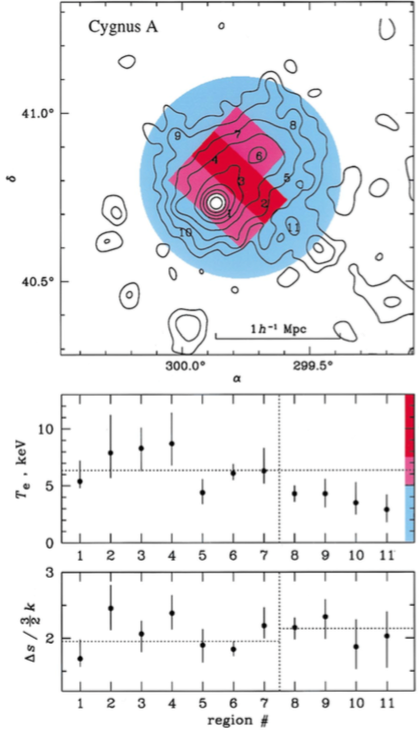
\includegraphics[width=0.78\textwidth]{introduction/xray/ASCA_TempMap.png}
\caption{\citet{1999ApJ...521..526M} present observational evidence for
         an ongoing merger in Cygnus~A with a simple merger geometry. Top:
         \satellite{ROSAT} PSPC \citep{1996MNRAS.278..479R} contours with
         \satellite{ASCA} temperature extraction regions numbered from 
         $1$ to $11$, where regions of similar temperature are colour-coded
         with the same colour. NB, the central region containing the central
         source Cygnus~A is omited. Middle: with numbers of extraction region
         on the horizontal axis, the vertical axis shows the corresponding
         temperature. The same colours used in the top panel are indicated
         in a bar on the right-hand side. Bottom: specific entropy. }
\label{fig:ASCA_TempMap}
\end{figure}

The best X-ray observations of Cygnus~A prior to the \citet{2014cxo..prop.4448W} study
are published by (I) \citet{2000ApJ...544L..27W}, (II) \citet{2002ApJ...564..176Y},
and (III) \citet{2002ApJ...565..195S}. The last two publications in this series of
three are titled `A \satellite{Chandra} X-ray study of Cygnus~A', followed by roman
numbering `II' or `III' and a sub-title indicating the scope. Paper II focusses on
the nucleus, while III focusses on the cluster of galaxies. Note that the title of 
the first paper is different as it starts with `Chandra Observations of Cygnus A' 
followed by the scope, which is the hot spots emission. We only consider
the third publication in this series as it focusses on the cluster emission. Most notably,
the authors suggest that the plume to the North West is associated with
an other (sub)cluster of galaxies and the total cluster mass is inferred under the assumption of 
hydrostatic equilibrium. Our results will be compared in detail with the quantitative results
of \citet{2002ApJ...565..195S} in chapter~\ref{sec:discussion}. Note that the
data obtained as part of this series of publications is included in our analysis too and
is referred to as `the archival data'.

The best optical observations of the cluster galaxies to date provide improvements to 
the previous optial study of \citet{1997ApJ...488L..15O}. Redshift measures of an additional
77 galaxies allows \citet{2005AJ....130...47L} to set up a dynamical model of the cluster.
The data are consistent with two sub clusters separated by \mytilde $700 \, h_{75}^{-1}$ kpc 
(x-ray) or \mytilde $460 \, h_{75}^{-1}$ kpc (optical, surface density peaks), a velocity 
separation between the sub clusters of $1600-2600$ km/s, and a virial mass ratio of $3:1$. 
The data is consistent with a merger either $0.2-0.6$ kpc prior to core passage, or 
$>2$ Gyr post-core passage. However, the high velocity dispersion measured strongly favours 
the pre-core passage scenario. The system is oriented on the sky with a projection angle of 
\mytilde $30^{\circ} - 45^{\circ}$. Bimodality in the updated velocity distribution histogram
(Figure~\ref{fig:velocityDispersion_2005}) is less significant than the previous study showed.
Furthermore, the X-ray gas and the optical galaxy distribution seem to align rather well 
(Figure~\ref{fig:velocityDistribution_2005}).

\begin{figure}
\centering
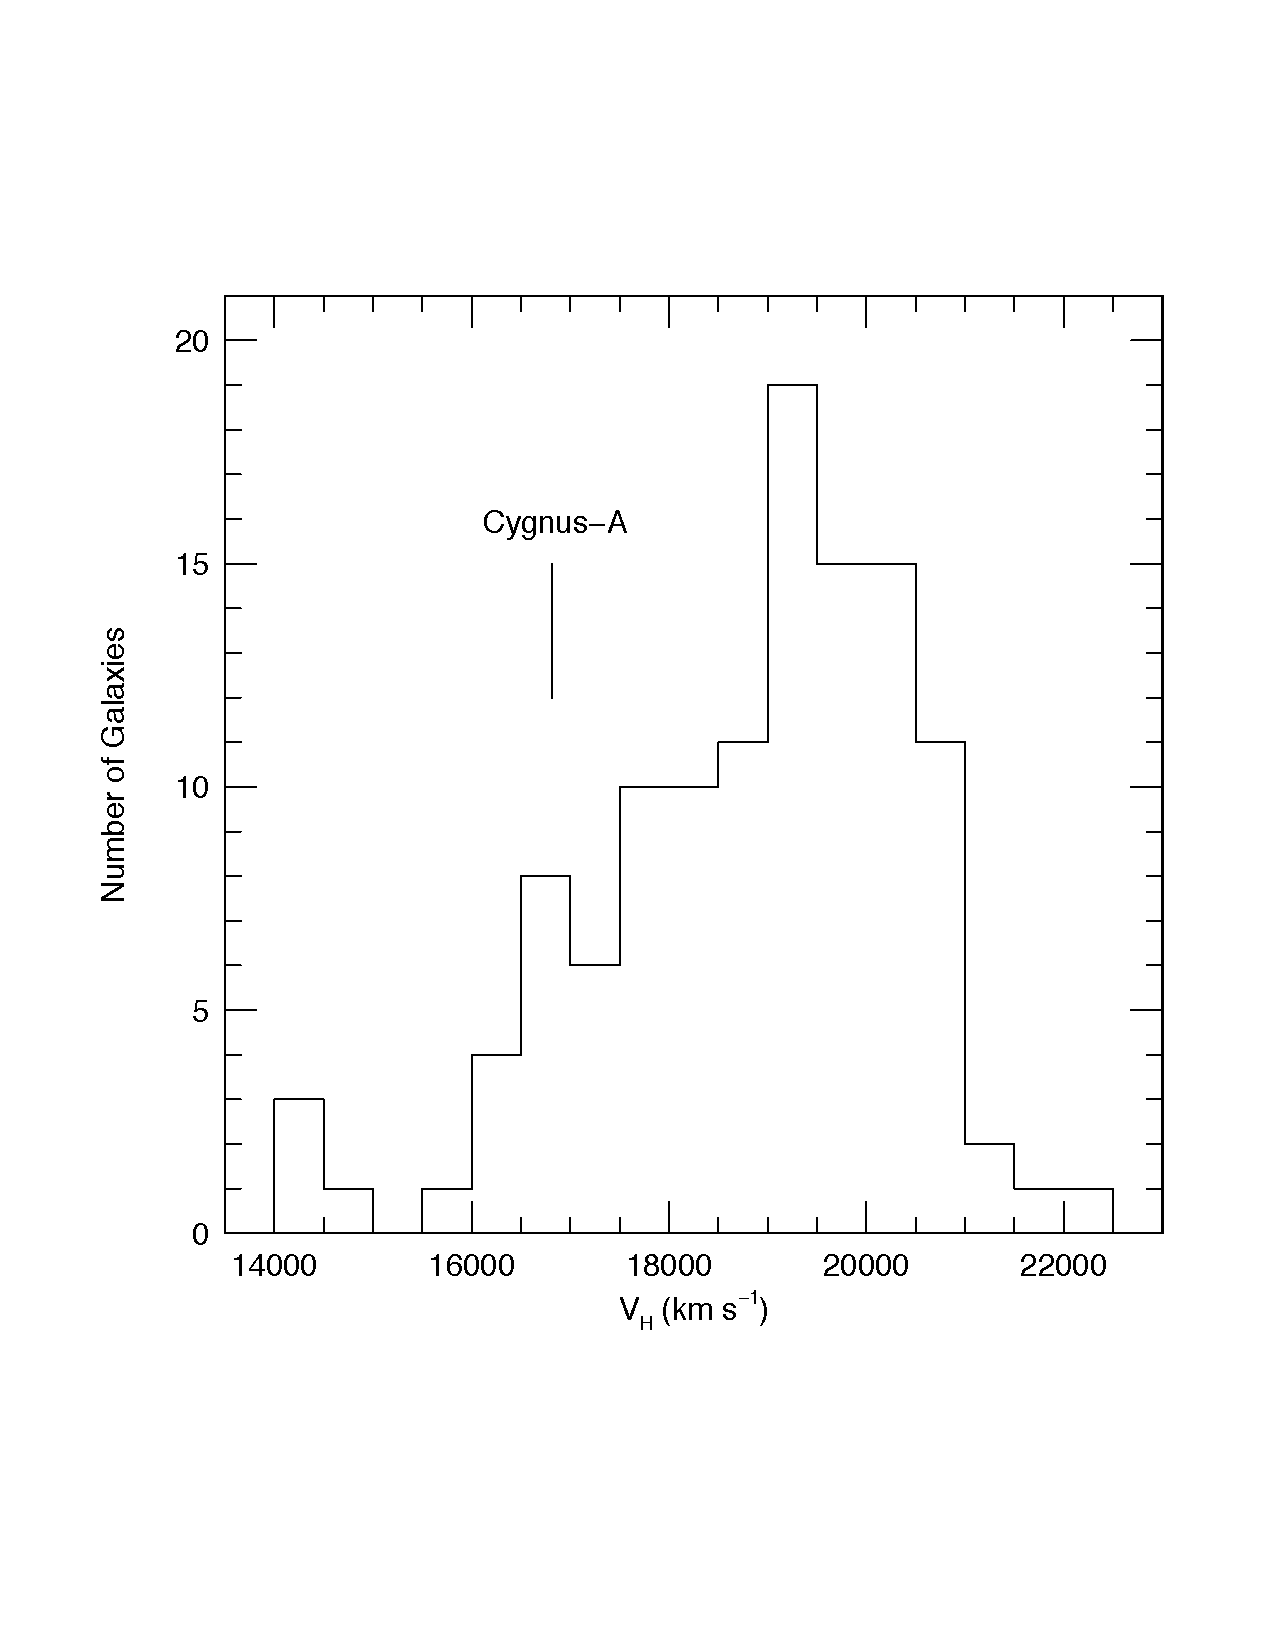
\includegraphics[width=0.74\textwidth]{introduction/optical/CygA_VelocityDispersion_2005.pdf}
\caption{Histogram showing the radial velocities obtained for 118 galaxies part of the 
         Cygnus~A cluster by \citet{2005AJ....130...47L}. The bimodality found earlier
         is less significant in this figure.}
         
\label{fig:velocityDispersion_2005}
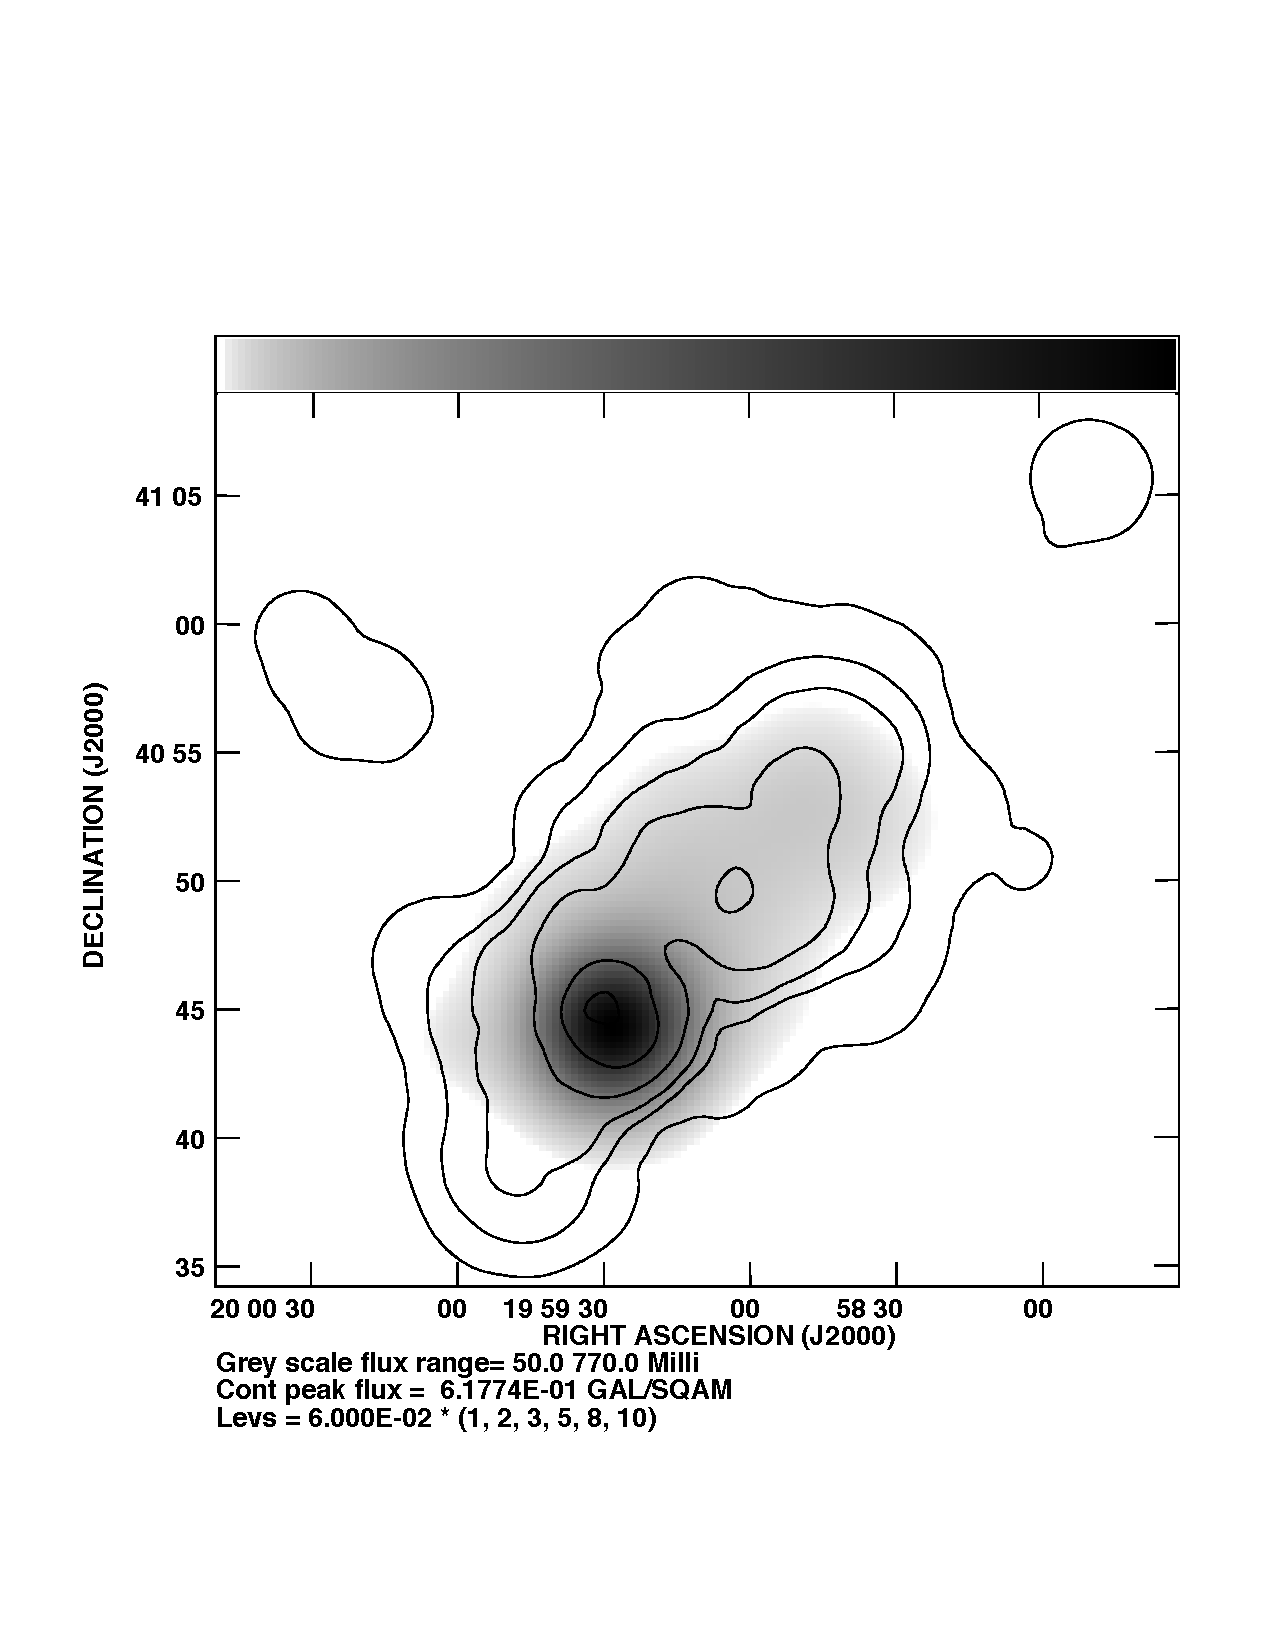
\includegraphics[width=0.7\textwidth]{introduction/optical/VelocityDistribution_2005.pdf}
\caption{The contour overlay shows the adaptively smoothed galaxy distribution
         centered on the dynamical center of mass overplotted on the \satellite{ROSAT}
         PSPC X-ray observation \citep{1996MNRAS.278..479R}. CygA is located at the
         brightest source of X-ray emission. Figure adopted from \cite{2005AJ....130...47L}.}
\label{fig:velocityDistribution_2005}
\end{figure}

The final publication to complete our literature overview shows a significant 
temperature jump (Figure~\ref{fig:Suzaku_MergerShock}) between the two sub 
clusters in \satellite{Suzaku} data \citep{2013AN....334..346S} The authors 
interpret this feature as a merger shock.

\begin{figure}
\centering
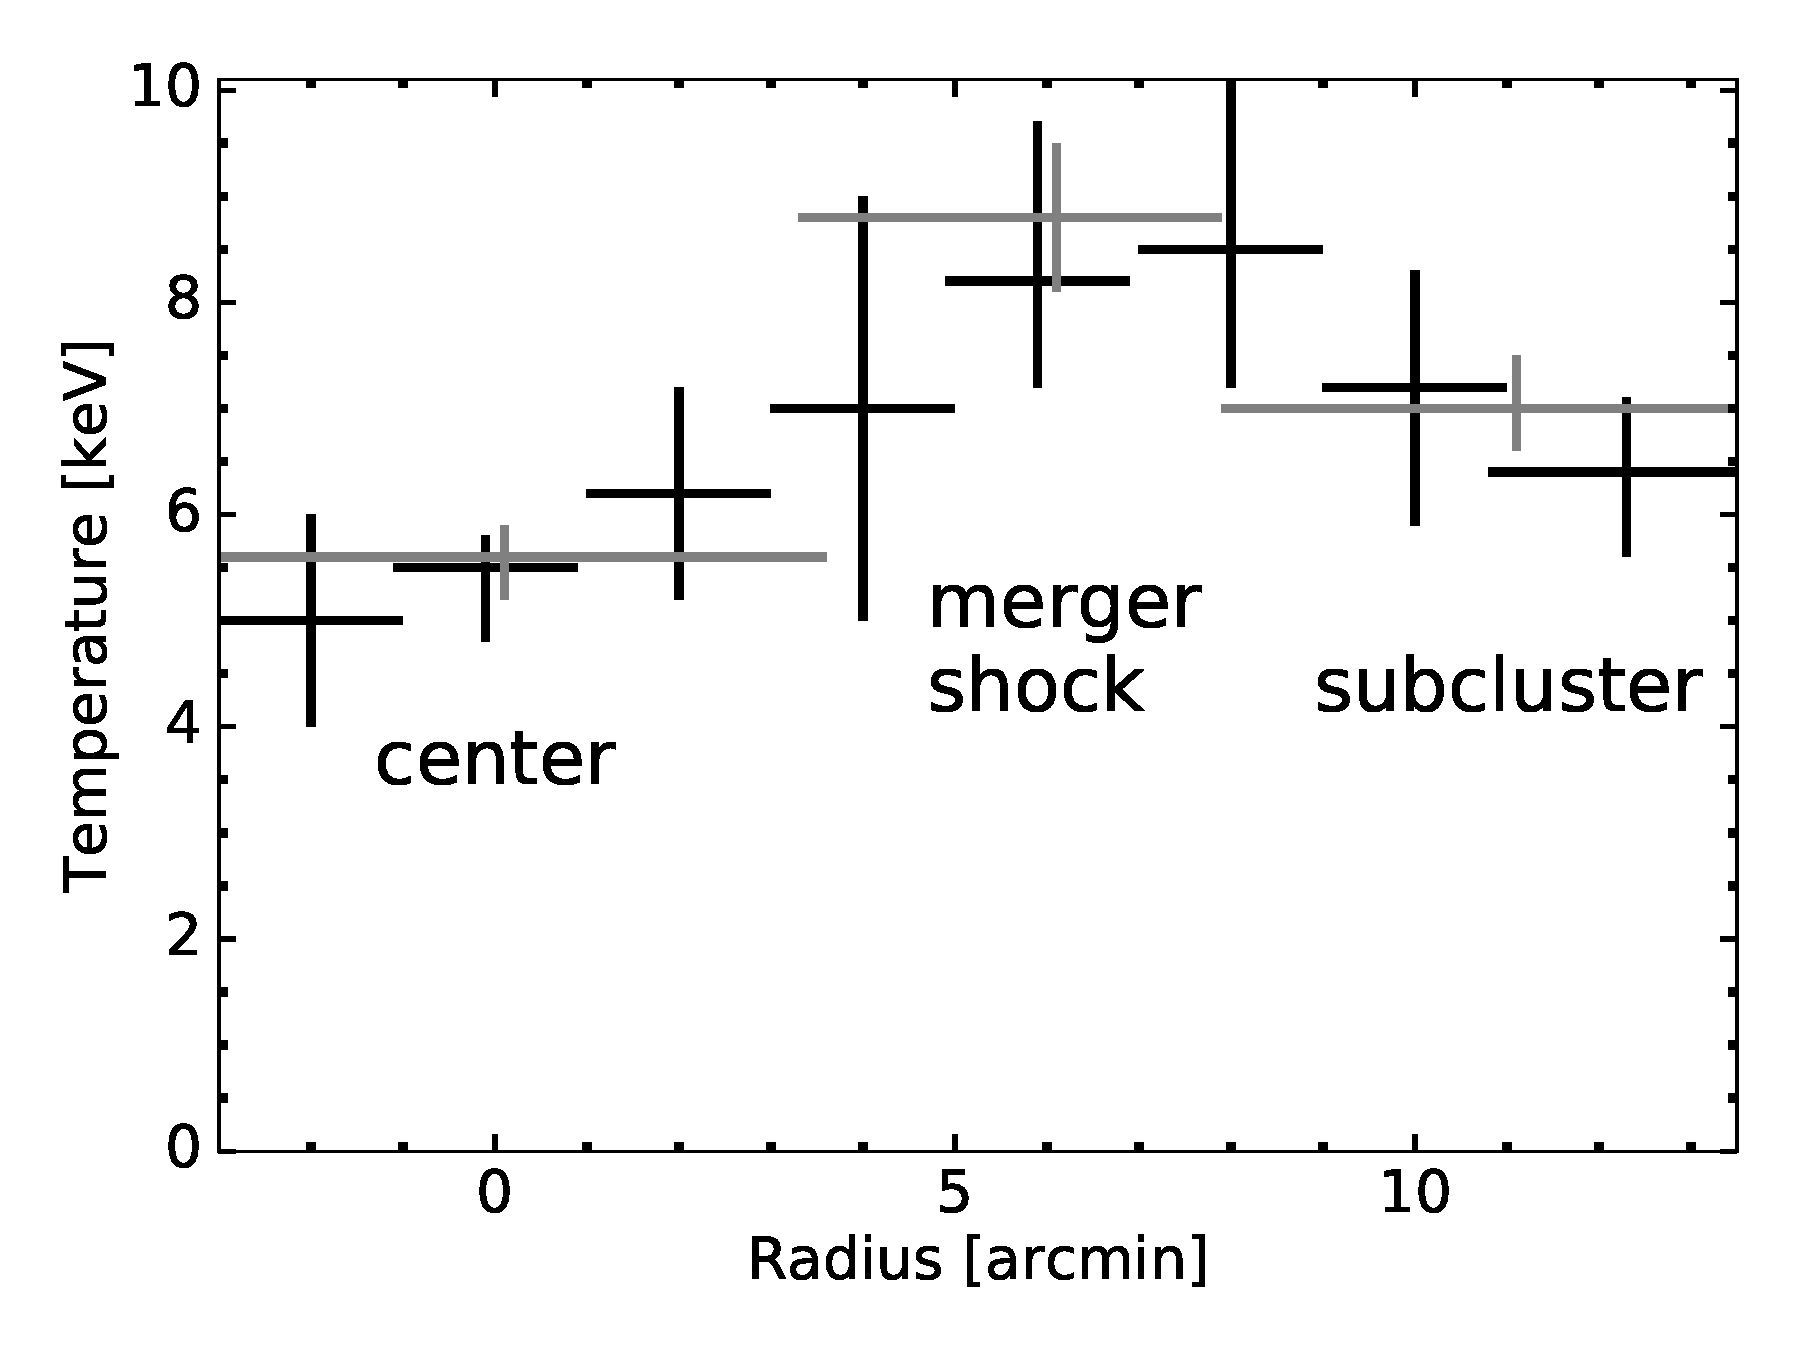
\includegraphics[width=0.6\textwidth]{introduction/xray/suzaku_temperaturejump.pdf}
\caption{\satellite{Suzaku} data shows a temperature jump between Cygnus~A and the
         sub cluster to the North West. Figure reproduced from \citet{2013AN....334..346S},
         who interpret this feature as a merger shock.}
\label{fig:Suzaku_MergerShock}
\end{figure}

\SubfileBibliography
\end{document}   
